\documentclass[tikz]{standalone}
\usetikzlibrary{calc,arrows}

\begin{document}
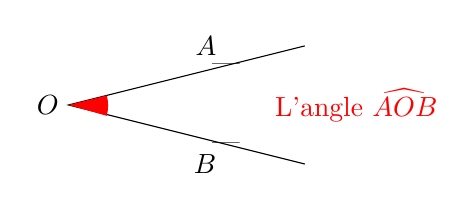
\begin{tikzpicture}
    \coordinate (O) at (0,0);
    \coordinate (A) at (2,0.5);
    \coordinate (B) at (2,-0.5);
    \draw ($(O)!1.5!(A)$) -- (O) -- ($(O)!1.5!(B)$);
    \fill[red] ($(O)!0.5cm!(A)$) arc (15:-15:0.5) -- (O) -- cycle;
    \node at (A) {|};
    \node[above left] at (A) {$A$};
    \node at (B) {|};
    \node[below left] at (B) {$B$};
    \node[left] at (O) {$O$};
    \node[anchor=west] at (2.5,0) {\textcolor{red}{L'angle $\widehat{AOB}$}};
\end{tikzpicture}
\end{document}